

Même si les prototypes sont bons, il y a pour l'instant peu d'analyse des proptotypes (on ne montre pas qu'il y a
un lien entre la conception et la fabrication du prototype) mais surtout il n'y a pas de retour vers le 
dimensionnement (pas d'analyse des observations faites sur le prototype). On s'attend à un retour vers le modèle
théorique pour voir s'il y avait lieu de suivre cette procédure de dimensionnement, c'est l'objectif du second 
quadrimestre.

\section*{Acquis du premier quadrimestre}
\begin{wrapfigure}[4]{r}{2cm}
\vspace{-12mm}
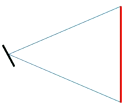
\includegraphics[scale=0.45]{ch1/image1.png}
\captionof{figure}{ }
\end{wrapfigure}
Nous avions établi via la procédure de dimensionnement (version simplifiée).
\begin{equation}
\theta_m = \dfrac{NB\ell L}{J_{tot}\omega^2}I_m
\end{equation}

\begin{wrapfigure}[7]{l}{4cm}
\vspace{-10mm}
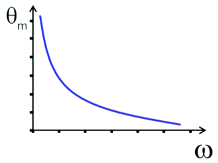
\includegraphics[scale=0.45]{ch1/image2.png}
\captionof{figure}{ }
\end{wrapfigure}
Une variation sinusoïdale du courant donne bien lieu à une variation sinusoïdale de la position donnée par
$\theta_m$ : celle-ci peut déjà être testée en pratique. Ci-dessus, on représente le prototype à une 
dimension dont l'amplitude peut directement être mesurée (trait rouge, en fonction de $\omega$) de façon à 
vérifier ce premier modèle. Le résultat attendu est une courbe en $1/\omega^2$ comme représenté 
ci-contre\footnote{Le schéma est simplifié, pour voir quelque chose on préférera un graphe logarithmique afin
d'obtenir une droite.}.\\

Ceci est bien sûr idéalisé, on ne doit pas s'attendre à avoir une si belle courbe : en rouge est représenté 
quelque chose de plus conforme à la mesure expérimentale et en particulier on peut y voir la présence d'une 
résonance\footnote{Il ne veut pas s'attendre à aller à plus de 1000 Hz dans notre système, l'étude se fera
bien en dessous de ce seuil.}. On peut s'attendre à cette résonance car le courant $I_m$ ne détermine que 
l'accélération angulaire de la bobine $\ddot{\theta_m}$ dans ce premier modèle et ceci car aucune perte 
n'avait été déterminée. Pour remédier à ceci, on préférera 
\begin{equation}
J_{tot} \ddot{\theta} = NB\ell LI_m\sin(\omega t) - \kappa\theta-\lambda\dot{\theta}
\end{equation}
où l'on voit apparaître une force de rappel ainsi qu'un frottement visqueux (d'autres modèles peuvent être
étudiés).\\


\begin{wrapfigure}[4]{r}{4cm}
\vspace{-16mm}
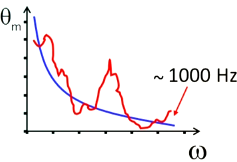
\includegraphics[scale=0.45]{ch1/image3.png}
\captionof{figure}{ }
\end{wrapfigure}
 La force de rappel permet de modéliser la \textit{dérive angulaire} qui, en faisant tourner la 
bobine dans le dispositif, fait souvent un bruit typique \textit{toc-toc} sur les parois du dispositif. Pour
éviter cette dérive, on essaye de maintenir la bobine autour d'une position d'équilibre afin d'éviter ces 
cognements. On peut pour ça disposer les fils de contacts (amenant le courant dans la bobine) afin de stabiliser
la position de la bobine : cela correspond à un certain \textit{coefficient de rappel angulaire} $\kappa$.\\

Le frottement doit également être pris en compte, modélisé par un visqueux en $\dot{\theta}$. On retrouve 
l'équation de l'OLAF avec notre terme de forçage harmonique. Ceci entrevoit bien la résonance mais il ne faut
pas pour autant que les étudiants calculent la solution analytique de cette équation différentielle car il 
faudrait maîtriser les phaseurs. Ils peuvent cependant prendre conscience des solutions de cette équation. \\

\begin{wrapfigure}[5]{r}{4cm}
\vspace{-15mm}
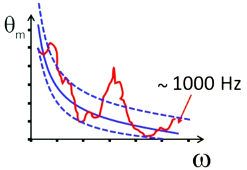
\includegraphics[scale=0.45]{ch1/image4.png}
\captionof{figure}{ }
\end{wrapfigure}
Une autre chose est l’influence du courant $I_m$. Il faut en effet voir si $\theta_m \propto I_m$. Si c'est le
cas, nous obtiendrons une translation verticale de la courbe précédemment mesurée comme suggéré ci-contre 
(il faudrait la représenter avec ses non-idéalités).\\

 Mais les BA1 ne seront pas capables de mesurer le 
courant de façon autonome : \textsc{Permanence technique} le 16 et le 17 février dont le but sera de faire cette
étude de l’influence du courant sur la position du faisceau laser via le dispositif suivant.


\begin{center}
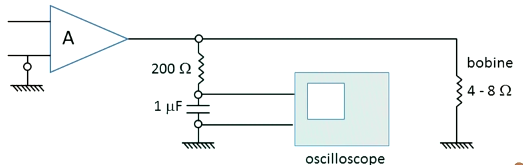
\includegraphics[scale=0.65]{ch1/image5.png}
\captionof{figure}{ }
\end{center}

On propose d'étudier le courant à partir de la tension appliquée à la bobine (qui présente une résistance de 
4 à 8$\Omega$). On s'intéresse à la tension aux bornes de notre bobine de sorte à en déduire le courant via
la loi d'Ohm mais on fait un peu plus compliqué en plaçant un filtre RC : il faudra prévoir deux points de
branchements (pinces crocodiles) pour tester le dispositif.\\

Les BA1 verront ceci dans leurs études, mais on ne demande pas le détail du fonctionnement du RC : ils doivent
sommairement le comprendre : le condensateur à une réactance en $1/(\Omega C)$ (intuitivement, si $\Omega=0$, 
tout se stabilise et se passe comme le cas du circuit-ouvert et donc résistance infinie. S'il n'y a pas de 
courant qui passe, on mesure la tension dans la résistance du dessus soit celle fournie par l'AOP.) signifiant
qu'en fréquence basse on mesure la tension appliquée à la bobine. A fréquence élevée, tout va se passer comme
si on avait un court-circuit et mesurer zéro à l'oscilloscope. On a bien un filtre \textit{passe-haut} qui est
nécessaire pour éliminer le bruit.\\

On peut ainsi relever le courant fourni à la bobine au travers de la tension appliquée à cette bobine avec une
fréquence coupure de $5 kHz$ du filtre. On va obtenir une courbe par courant donné. Mais qu'est ce qu'ils peuvent
apprendre de cette courbe\footnote{Notons que la résonance ne sera pas forcément visible, dans le cas où le 
frottement est assez important.} ? On va supposer que le prototype ne s'écarte pas trop de notre modèle 
théorique.\\


\begin{wrapfigure}[5]{r}{4cm}
\vspace{-15mm}
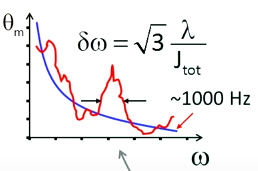
\includegraphics[scale=0.45]{ch1/image6.png}
\captionof{figure}{ }
\end{wrapfigure}
La résonance est donnée via l'équation de l'OH
\begin{equation}
J_{tot} \ddot{\theta} + \kappa\theta=0\qquad\Leftrightarrow\qquad \omega_0 = \sqrt{\dfrac{\kappa}{J_{tot}}}
\end{equation}
Ce qui nous permet de déduire $\kappa$. De même, l'étude de la largeur de la résonance $\delta \omega$ donné
par
\begin{equation}
\delta\omega = \sqrt{3}\dfrac{\lambda}{J_{tot}}
\end{equation}
nous permet de déduire la valeur du paramètre $\lambda$. Tout ceci est laissé à caution (on ne sait pas si elle
va apparaître) mais si c'est le cas on parvient à mieux caractériser le système mais il ne faut \textbf{pas} 
demander aux étudiants de s'attaquer à la théorie des phaseurs. Une ouverture du syllabus aux pages de l'analyse
de la résonance suffit. Ceux qui n'observent pas de résonances pourront en tirer la conclusion d'un amortissement,
par exemple, trop important et que la résonance est invisible.\\

\begin{wrapfigure}[6]{r}{4cm}
\vspace{-5mm}
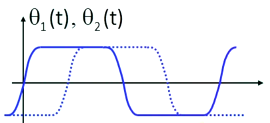
\includegraphics[scale=0.45]{ch1/image7.png}
\captionof{figure}{ }
\end{wrapfigure}
Le but du second quadrimestre est d'obtenir une maîtrise suffisante pour représenter des motifs 2D sur un écran, 
tel un carré. Pour le dessiner, il faut jouer sur les variations des angles $\theta_1(t), \theta_2(t)$ qui n'est
rien d'autre que la paramétrisation. On pourrait considérer la variation représentée ci-contre (quadrature) pour dessiner ce beau carré. Il s'agit bien de la paramétrisation du carré, il faut ensuite faire en sorte que les 
angles bougent de cette manière mais cela ne veut pas dire que le courant doit suivre exactement cette courbe. 
Nous avions
\begin{equation}
I_1(t) = \dfrac{J_{tot}}{NB\ell l}\ddot{\theta_1}
\end{equation}
Qui informe sur le lien entre l'\textit{accélération angulaire} et le courant. On pilote le prototype en une 
accélération qui est proportionnelle au courant. Pour trouver le courant correspondant à la formation du carré, 
il faut dériver deux fois les angles
\begin{center}
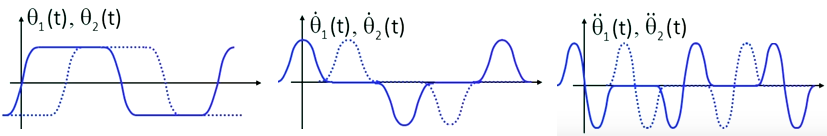
\includegraphics[scale=0.5]{ch1/image8.png}
\captionof{figure}{ }
\end{center}
Le courant doit être proportionnel au signal tout à droite pour pouvoir dessiner un carré, le courant donne 
l'accélération! Pour monter la première face du carré (côté Ouest) il faut accélérer puis décélérer. Le problème
c'est que le modèle dynamique est plus compliqué
\begin{equation}
I_1(t)= \dfrac{1}{NB\ell L}[J_{tot}\ddot{\theta_1}+\lambda\dot{\theta_1}+\kappa\theta_1]
\end{equation}
On voit alors qu'il n'est pas nécessaire de résoudre cette équation car on veut connaître la valeur d'un courant
donné pour une valeur de $\theta_1$. Il ne faut \textbf{pas} confronter les étudiants à la résolution de cette
équation car, encore une fois, on ne cherche pas $\theta_1$ mais $I_1(t)$. Nous on veut \textit{connaissant 
$\theta_1$, qu'est ce qu'il faut envoyer comme courant dans le dispositif} et nous, on connaît $\theta$ sur 
base de la figure que l'on veut réaliser. On utilisera le premier et le second graphique ci-dessus pour tenir
compte du frottement et de la force de rappel.































